\chapter{Search for X17}
\begin{refsection}
\label{ch:X17}
{\itshape After the recent publications from the ATOMKI collaboration, the so-called X17 anomaly piqued the interest of the community. The flexibility of the MEG II apparatus allows for a variety of exotic searches and the collaboration deemed of interest in searching for this anomaly in an uncorrelated way.
The chapter starts with a recap of the previous searches and then moves to the description of this search in MEG II: setup used, simulations developed, data acquisition, and data analysis.}

\section{ATOMKI and the X17 `anomaly'}
    In recent years, the nuclear reaction \ce{^7Li(p,\e,\Ae)^8Be} peaked the physics community's interest.
    The reason is, in 2016 the Atomki laboratory reported an excess in the angular distribution of the pairs $\e \Ae$ coming from the Internal Pair Creation (IPC).
    The significance found was $\approx7\sigma$ and similar results were later obtained.
    The current explanation is the creation of a \SI{17}{MeV/c^2} boson (hence the name), associated with the interaction of dark and ordinary matter.

\status{started}
\section{X17 in MEG II}
    After reading with great interest the papers from ATOMKI, the MEG collaboration started evaluating if repeating this measurement was achievable with the MEG II apparatus.
    In 2022 the first data collection was performed but the time constraints, required to keep the main focus of the experiment on the $\upmu \rightarrow \upgamma e$ process, meant not all the necessary preparatory studies could be performed.
    The details of this first data-taking will be skipped and we will move directly to the second campaign, performed in 2023.
    
    \subsection{MC simulations}
    
    \status{started}
    \subsection{Magnetic field choice}
        The first step is to identify the magnetic field required. 
        The geometry of the MEG II detector, in junction with the magnetic field, defines the acceptance of the produced particles.
        Given the nature of the COBRA magnet, the parameter here is the scaling of the magnetic field.
        Thorough simulations were run to optimize the scaling factor, finding the best compromise between the efficiency for signal and background reconstruction to be $B_{X17}=0.15\times B_{MEG}$. 
        This value can be roughly estimated considering that a scale factor of 1 is optimized for positrons of \SI{53}{MeV} while the pair produced by the X17 decay should be roughly at \SI{8}{MeV} ($8/53\approx 0.15$). 
        
    \status{started}
    \subsection{Target}
        The setup for the target is quite straightforward: a carbon fiber vacuum chamber is mounted at the tip of the insertion system of the CW bellows system; a mounting system holds different types of targets.
        The bellows system is the one used for XEC weekly calibrations and will be not discussed.
        
        \paragraph{Vacuum and mechanical structure}
        The thickness and dimensions of the carbon fiber vacuum chamber have been optimized via dedicated simulations for both integral structure and particle interaction.
        After receiving the carbon fiber, the chamber was glued and tested for vacuum.
        
        \paragraph{Lithium targets}
        The interesting process requires Lithium atoms but Lithium targets tend to be unstable. 
        Among the options studied \ce{LiF} and \ce{Li_{3.6}PO_{3.4}N_{0.6}} were the most promising.
        \ce{LiF} targets were produced by INFN Legnaro while \ce{Li_{3.6}PO_{3.4}N_{0.6}} targets were produced at PSI.
        Looking back we now know that the spattering process behind the production of the \ce{Li_{3.6}PO_{3.4}N_{0.6}} targets resulted in a poorly characterized end-product (more on this in a following section).
        What drove us to rely on the LiPON instead of the LiF was to avoid the F resonance. 
        More on targets will follow.
        
\status{started}
\section{Data acquisition}
    We went through two short data-taking periods. 
    The first was at the end of 2022 and lasted 3 weeks while the second was in Feb. 2023 and lasted 4 weeks.
    During the first period, we collected data used to develop the MC simulations, event reconstruction, and optimize the trigger.
    At this stage, the understanding was only partial but we deemed it sufficient to collect useful data as an intermediate step.
    The second period was the main data acquisition. 
    
    \status{review}
    \subsection{Beam tuning}
        The beam tuning was performed by substituting the end cap of the proton beam line with a transparent cap with a AAA crystal. 
        The proton beam produces visible photons hitting the crystal so the beam position can be observed.
        Normally this operation would be done while the upstream side of COBRA is not closed, allowing the installation of a webcam that gives instant feedback on the beam position.
        This was not the case so we were forced to use the camera installed inside COBRA for MEG II target monitoring.
        This camera has some settings for \textit{gain} and \textit{aperture} but is controlled using a script in \textit{ssh} and to view the picture first is necessary to move them locally, making the whole procedure somewhat cumbersome.
        Key aspects of the beam to be tuned were: 
        \begin{outline}
            \1 Energy: This parameter is controlled by the \textit{Terminal Voltage} of the CW.
            \1 Focus: This parameter is controlled by the \textit{Extraction Voltage} of the CW. Fig.~\ref{fig:focus_500keV} shows how the beam spot changes as a function of this parameter. 
            \1 Position: This parameter is controlled by the three dipoles of the CW beamline. The change of the position for different values of the dipoles at \SI{500}{keV} is shown in Fig.~\ref{fig:position_500keV}.
        \end{outline}

        \begin{figure}
            \centering
            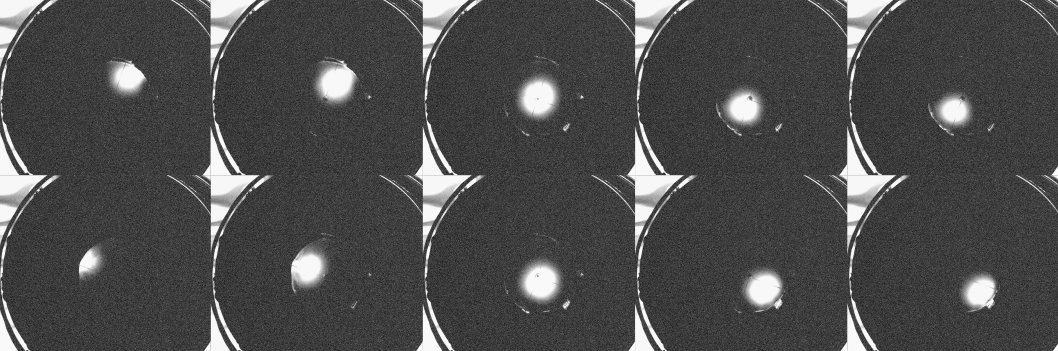
\includegraphics[width = \textwidth]{Figures/X17/beamtuning/psotion_500keV.png}
            \caption{Position of the proton beam at \SI{500}{keV} when changing the current in the dipoles (the vertical dipole V and only one of the two horizontal dipoles H). In the first row, H is changing and the beam moves diagonally. In the second row, V moves the beam on the perpendicular diagonal.}
            \label{fig:position_500keV}
        \end{figure}
        \begin{figure}
            \centering
            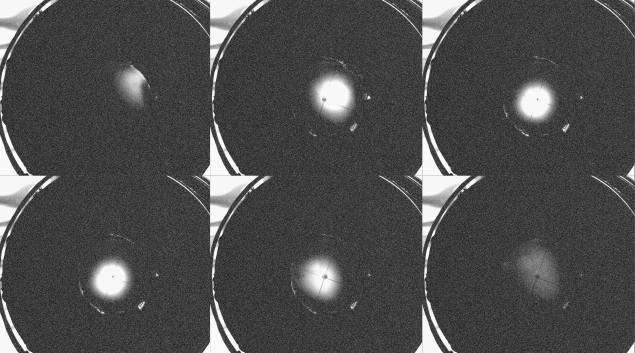
\includegraphics[width = \textwidth]{Figures/X17/beamtuning/focus_500keV.png}
            \caption{Focus of the proton beam at \SI{500}{keV} when changing the \textit{extraction voltage} of the CW: values in the range $6\divisionsymbol15$ keV. Is clearly visible for extreme values the beam barely reaches the crystal.}
            \label{fig:focus_500keV}
        \end{figure}
        \noindent
        After a careful scan of the three parameters, working points at different energies were chosen: the most relevant are the ones for \SI{500}{keV} and \SI{1080}{keV}.
        It is of interest to notice that \SI{1080}{keV} is the balance between what was previously discussed and the limitations of the CW machine: a higher ($\sim$\SI{1100}{keV}) energy would be a better choice but the nominal upper limit of the machine is \SI{1}{MeV}, meaning having it running stably at \SI{1080}{keV} is already an achievement.
        To the best of our knowledge, the beam at COBRA center during the data-taking was Gaussian \colorbox{red}{$(x, y) = \SIlist{2; -2}{mm}$; $(\sigma_x, \sigma_y) = \SIlist{2; 2}{mm}$}.

    \status{started}
    \subsection{Asymmetry and normalization}
        Important aspects to be considered during this search are the different asymmetries expected for the photons resulting from the interaction and the fact that our analysis will require a normalization measurement to keep track of the proton beam intensity.
        For the first task, the obvious choice would have been the XEC but this had two drawbacks: the detector itself is quite limited in extension along the beam direction and it was not always available due to the annealing process described in Sec.~\ref{sec:MEG:XEC}.
        The solution was to use the BGO, described in Sec.~\ref{sec:LH2:BGO}, and crosscheck the results via a dedicated data set collected with the XEC.
        For the normalization, the idea was to install a small NaI crystal below COBRA and use the combined information from this detector, the BGO, and the various measurements of the CW proton current.

\status{started}
\section{Data analysis}
    My contribution to the data analysis was only partial so I will not go into much detail. 
    Even so, at least a broad overview of the analysis status at the time of writing is in order.
    Most of the studies on event reconstruction and quality cuts were performed by Hicham Benmansour, while the Likelihood analysis was developed by Giovanni Dal Maso. 
    I contributed to the analysis of the BGO data and the development of the Likelihood analysis.
    
    \status{started}
    \subsection{Pair reconstruction}
        The first step for this search is to correlate particles and create $\e \Ae$ pairs. 
        This is not a given in an experiment that was developed for a different task, namely reconstructing $\e$ and $\g$. 
        The idea was, of course, to adapt the existing reconstruction code to the new aim.
        
        \paragraph{\textbf{B} inversion}
        As well known, particles of opposite charge behave symmetrically in the same B field.
        This means the $\e$ reconstruction in $\textbf{B}=B\hat{z}$ is equivalent to reconstructing a $\Ae$ in $\textbf{B}=-B\hat{z}$.
        This is a simple change to apply to the reconstruction code but holds only in the assumption the two particles behave in the same way while interacting with the different parts of the experiment.
        
        \paragraph{Vertexing}
        Once the reconstruction has been run on every event for both directions of magnetic fields, pairs need to be created.

    \status{started}
    \subsection{Feldman-Cousin}
        Although the Feldman-Cousin approach is well-established in particle physics research, this was our first hands-on experience. 
        After studying the relevant papers (\cite{feldman:1998}\cite{feldman:2011}) and the internal notes of the collaboration we decided to develop a mock-up experiment to understand the framework necessary for a Feldman Cousin approach to data analysis.  
        Given a measured sample and the probability density functions (PDFs) the framework we developed allows us to perform the analysis and obtain the confidence intervals.
        The full-blown X17 analysis was actually performed with the code already written for the MEG II analysis. This code was developed and improved upon over many years and was both more robust and flexible. 
        Although it was an `academic exercise', this effort made understanding the existing code and the underlying theory/structure an easier task.  
        I contributed actively to this effort until we managed to have a running structure.
        Although I followed the whole procedure, the finalization of the mockup\footnote{ The full description of the code will be here skipped but it can be found in the following 
        \href{https://github.com/gdalmaso96/X17_LL_mock_up}{\underline{git repository \faGithubSquare}}} and the transition to the MEG II code was done by Giovanni Dal Maso.

        \paragraph{Likelihood}
        This is an exercise to build confidence level belts based on Feldman-Cousins ranking using binned data.
        The data is synthetic and composed of an exponential background with a fixed slope and a Breit-Wigner with unknown mass and width. The data is binned.
        For such analysis, the likelihood can be written as:
        \begin{equation}
            \mathcal{L}(\textbf{x}|\hat{\mathcal{N}}_{S}, \hat{\mathcal{N}}_{BK}, \hat{m}, \hat{\Gamma}) = \frac{\hat{\mathcal{N}}^\mathcal{N} e^{-\hat{\mathcal{N}}} }{\mathcal{N}!} \prod_{i=1}^{m} \Big( \frac{\hat{N}_S}{\hat{\mathcal{N}}} \hat{\pi}_{S, i} + \frac{\hat{N}_{BK}}{\hat{\mathcal{N}}} \hat{\pi}_{BK, i} \Big)^{\mathcal{N}_i}, \quad \hat{\mathcal{N}} = \hat{\mathcal{N}}_{S} + \hat{\mathcal{N}}_{BK}, \quad \mathcal{N} = \mathcal{N}_{S} + \mathcal{N}_{BK}
        \end{equation}
        Where $\mathcal{N}$ is the number of measured events, $\hat{\mathcal{N}}$ is the center of the Poisson distribution and $\mathcal{N}_i$ is the number of events in the $i$-th bin.
        The $\hat{\pi}_i$ variables are uniquely determined by the signal and background PDFs, and are the expected values of the fraction of events in the $i$-th bin.

        \paragraph{PDFs}
        The signal PDF is defined as a Breit-Wigner:
        \begin{equation}
	   \mathcal{S}(m | \hat{m}, \hat{\Gamma}) = \frac{k}{(m^2 - \hat{m}^2)^2 + \hat{m}^2\hat{\Gamma}^2}
        \end{equation}
        with:
        \begin{equation}
	   k = \frac{2\sqrt{2}\hat{m}\hat{\Gamma}\gamma}{\pi\sqrt{\hat{m}^2 + \gamma}}, \quad \gamma = \sqrt{\hat{m}^2 ( \hat{m}^2 + \hat{\Gamma}^2)}
        \end{equation}
        Given $\mathcal{S}(m | \hat{m}, \hat{\Gamma})$, it is possible to evaluate the $\hat{\pi}_{S,i}$:
        \begin{equation}
	   \hat{\pi}_{S,i} (m_i) = \int_{m_i - \Delta m}^{m_i + \Delta m} \mathcal{S}(m\prime | \hat{m}, \hat{\Gamma}) dm\prime
        \end{equation}
        with $\Delta m$ being the bin width.
        The background PDF is defined as an exponential tail:
        \begin{equation}
	   \mathcal{B}(m) = \lambda e^{-\lambda m}
        \end{equation}
        with $\lambda$ fixed.
        Given $\mathcal{B}(m)$, it is possible to evaluate the $\hat{\pi}_{BK,i}$:
        \begin{equation}
	   \hat{\pi}_{BK,i} (m_i) = \int_{m_i - \Delta m}^{m_i + \Delta m} \mathcal{B}(m\prime)  dm\prime
        \end{equation}
        with $\Delta m$ being the bin width.

        \paragraph{Toy MC framework}

    \status{started}
    \subsection{Asymmetry}
        After developing the necessary tools, the first step was to extract the information on the asymmetry to evaluate the `purity' of the data collected.
        
        \paragraph{BGO}
        \paragraph{XEC}

        \noindent
        The results from this analysis seem to indicate something was not well under control.
        We had few hints but most seemed to point towards some defect of the target. 
        Before moving on with the X17 analysis, we decided to follow these hints.
        
    \section{Measurement of the different targets}
        To further understand the results of the preliminary analysis, and to cross-check different hypotheses, a few of the targets were brought to different experts.
        \begin{outline}
            \1 Two of the LiPON targets were brought to the chemistry department in PSI. The first step was to cut the target and study it with an electron microscope.
            The result is shown in Fig.~\ref{fig:X17:target:LiPON:psi}.
            The target under study was produced at PSI and was supposed to be \SI{2}{\micro m} LiPON deposit on a Cu substrate.
        \end{outline}
        \begin{figure}
            \centering
            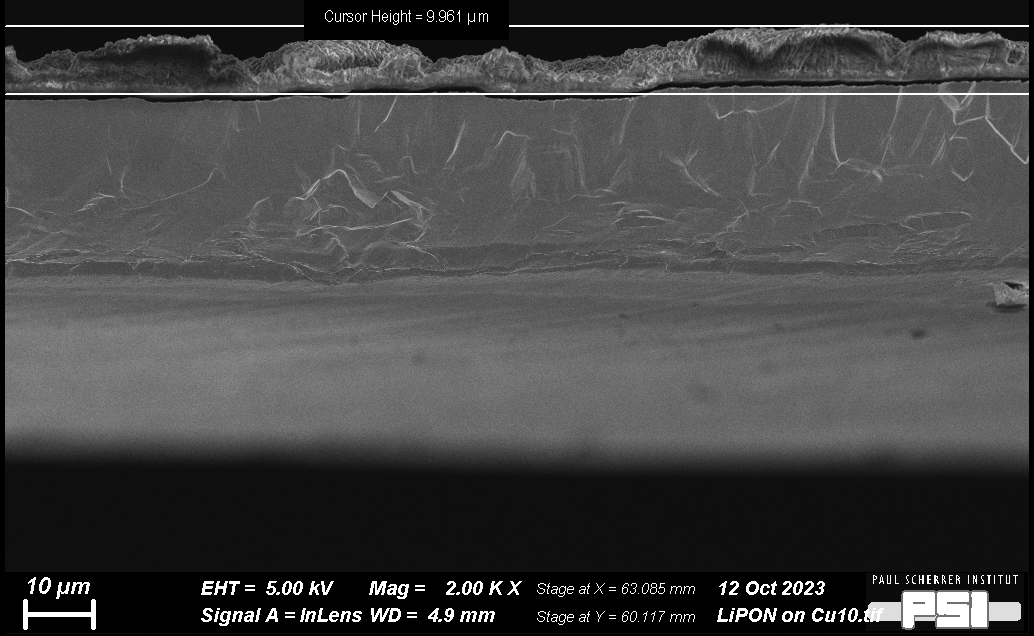
\includegraphics[width = 0.9\textwidth]{Figures/X17/PSI_LiPON_picture.png}
            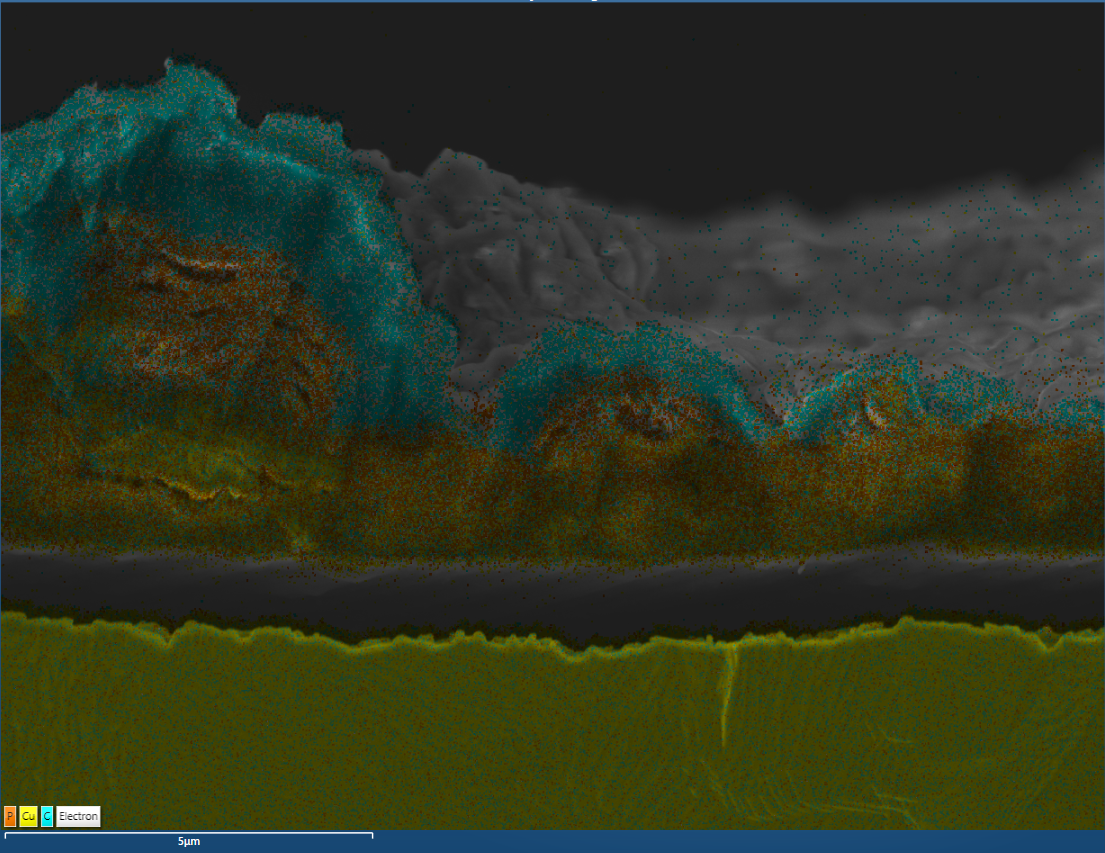
\includegraphics[width = 0.9\textwidth]{Figures/X17/PSI_LiPON-atoms_picture.PNG}
            \caption[SEM EDX LiPON analysis]{SEM and EDX measurement of the \ce{Li3PO4N2} deposit on the Cu substrate. For this particular target, the LiPON deposit was supposed to be \SI{2}{\micro m}. In the top picture, the LiPON rests on the copper substrate. In the bottom picture, the colors highlight the different atoms: Cu-yellow, P-orange, C-cyan. The presence of carbon is linked to the oxidation of the material, creating \ce{LiPO4}. The lamination between LiPON and Cu was attributed to the cutting procedure for the analysis.}
            \label{fig:X17:target:LiPON:psi}
        \end{figure}

\status{started}
\section{Target studies: Dec 2023}
    After the analysis done on the target used in Feb. during the data-taking, we asked some colleagues from PSI to produce a different LiPON target.
    The requirement was a target `as big as possible' and with a thickness of \SI{500}{\nano m}.
    The way the machine works made it so that the maximum dimension of the target was a diameter of \SI{1}{cm}.
    Given the setup developed for the target was for bigger substrates we had to improvise ways to hold this new target in position.
    We first tried to hold it between two folded aluminum foils. 
    This system was not satisfactory so we moved to a Cu foil with two parallel cuts to create a `pocket'.
    
    \subsection{Al Data-taking}
    \subsection{Cu Data-taking}
    
    \begin{figure}
        \centering
        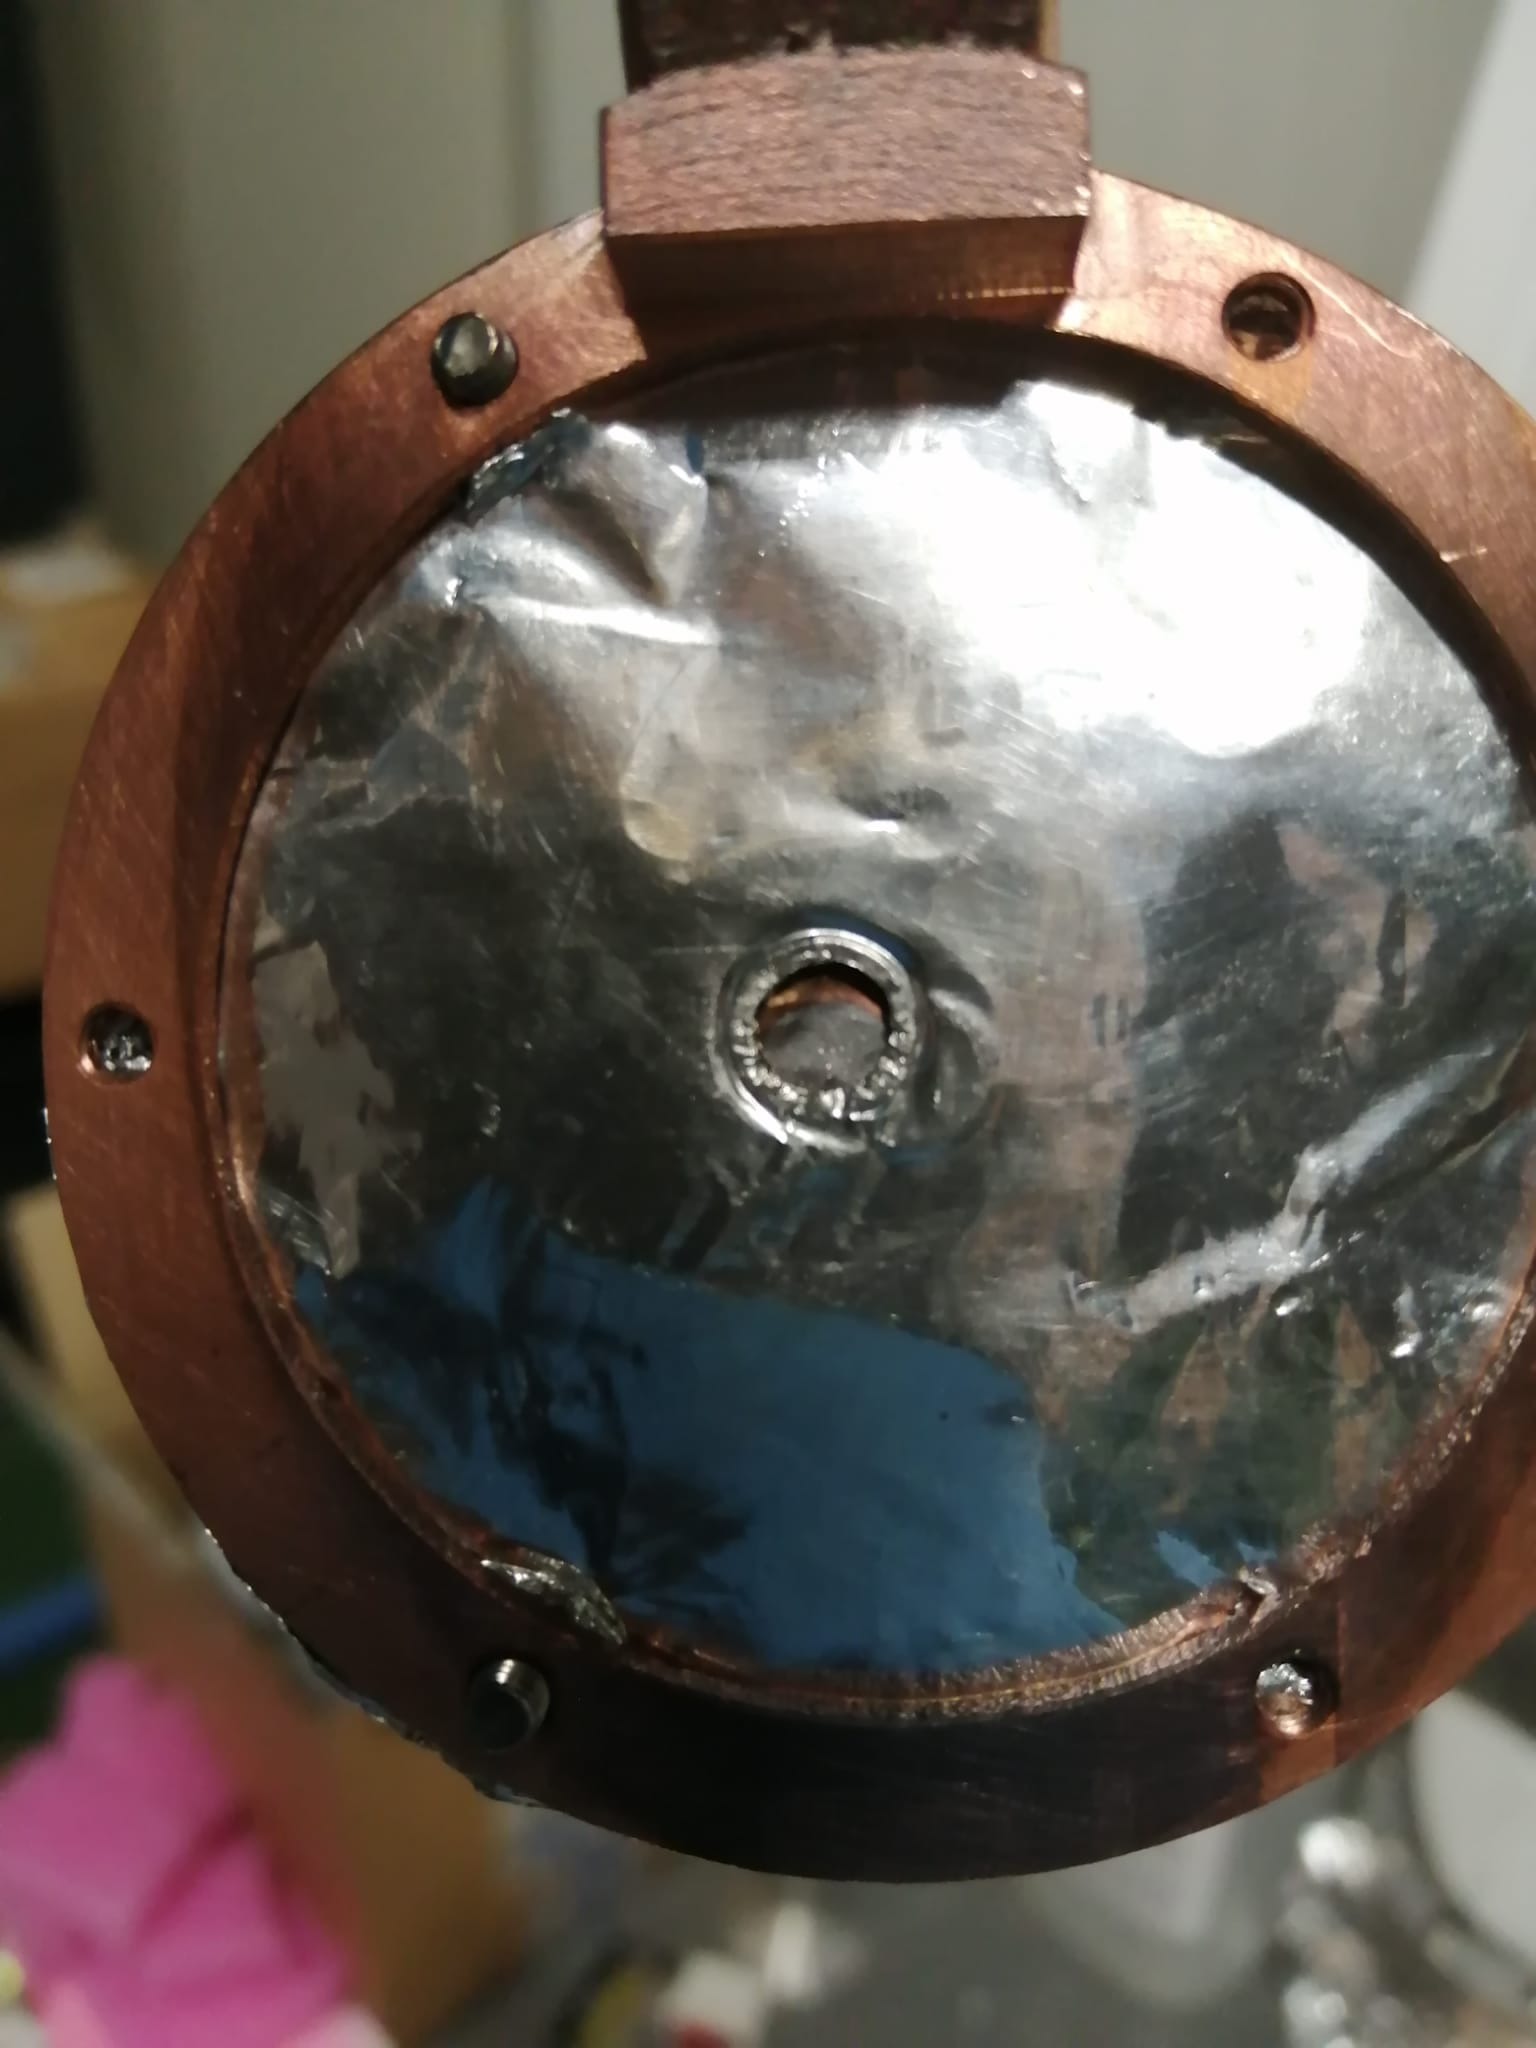
\includegraphics[width = 0.4\textwidth]{Figures/X17/Dec2023/X17_Dec2023_AlTarget.jpeg}
        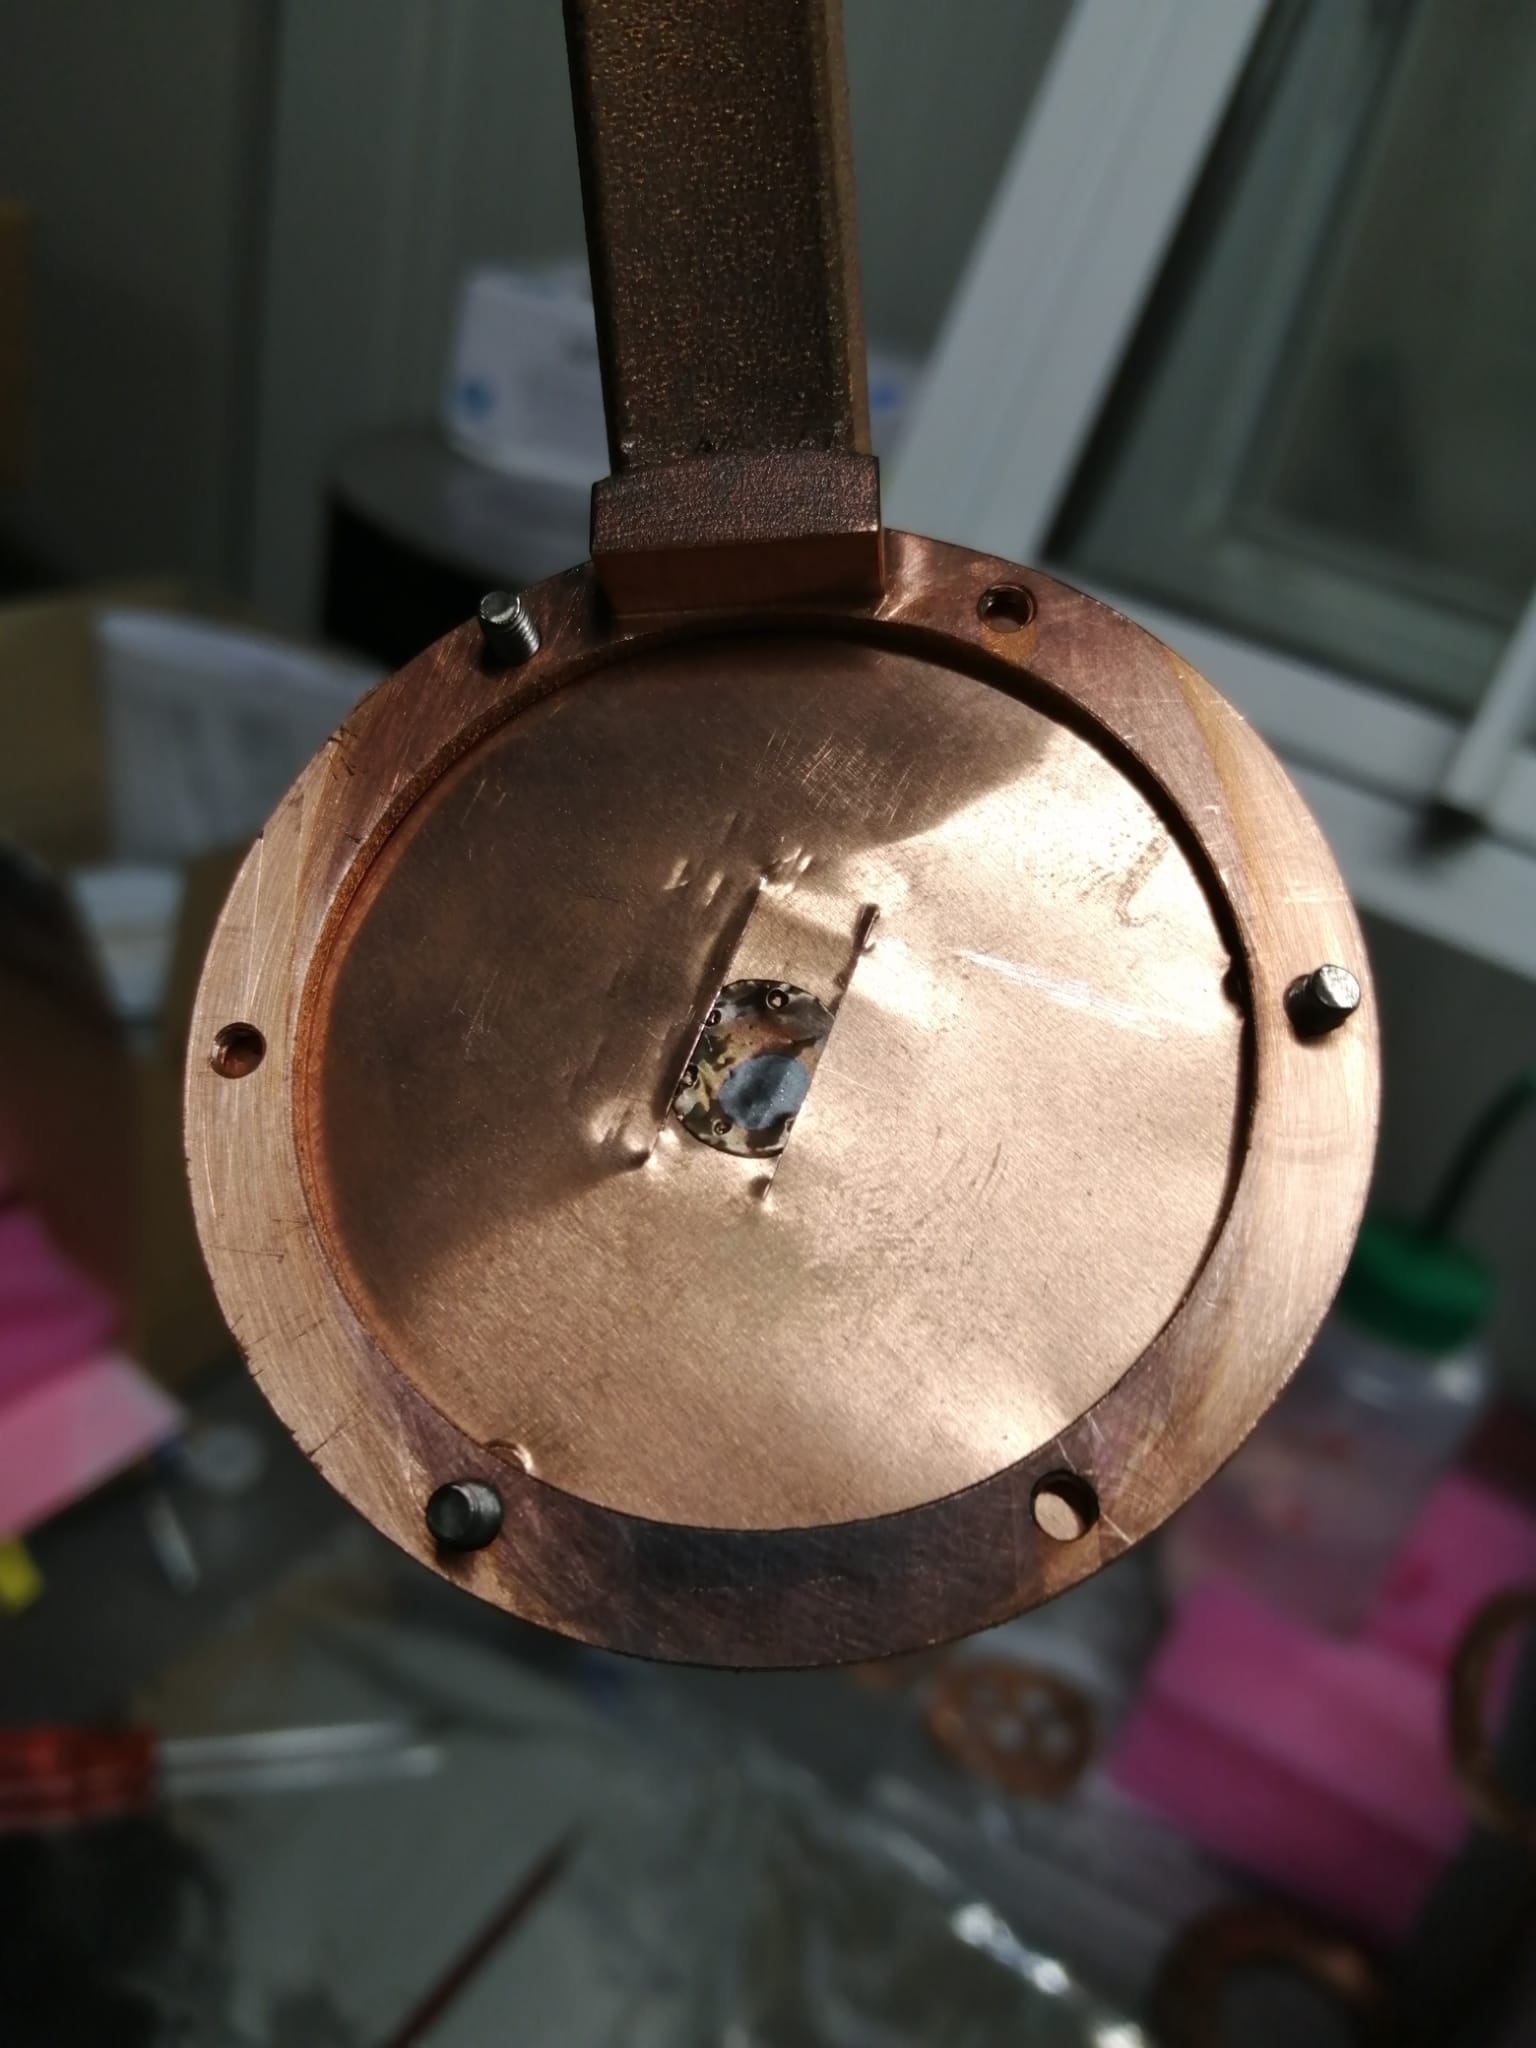
\includegraphics[width = 0.4\textwidth]{Figures/X17/Dec2023/X17_Dec2023_CuTarget.jpeg}
        \caption[Small LiPON target setup]{Two different ways to hold the small LiPON sample given to us by the PSI colleagues. We first tried to hold it in place with folded aluminum foils. We later realized this was not the optimal solution given the spectrum produced by protons on Al. We then moved to a cleaner Cu setup.}
        \label{fig:X17:target:LiPON:psi}
    \end{figure}
    \begin{figure}
        \centering

        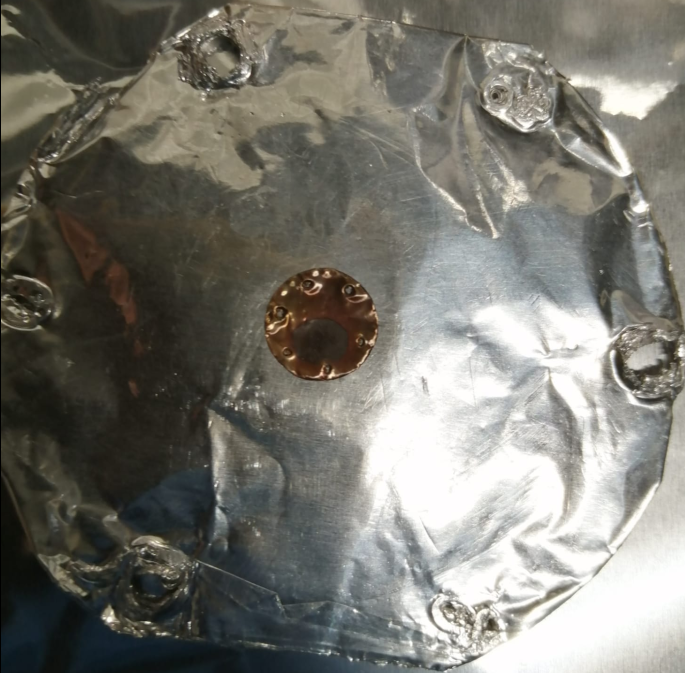
\includegraphics[width = 0.4\textwidth]{Figures/X17/Dec2023/X17_Dec2023_AlTarget_burned.png}
        \caption[Small LiPON target]{Here is a picture of the target itself after two days of datataking at 5 and \SI{10}{\micro A}. The dark spot marks the position on which the beam was impinging.}
        \label{fig:X17:target:LiPON:psi}
    \end{figure}       
\section{Beam studies: Jan 2024}

\section{Results and conclusions}

\cite{X17:1996} \cite{X17:nuclear:2004} \cite{X17:Krasznahorkay:2015} \cite{X17:Ellwanger:2016} \cite{X17:Feng:2016} \cite{X17_Kozaczuk:2017} \cite{X17:Krasznahorkay:2017} \cite{X17:2019} \cite{X17:2021} 

\status{started}
\printbibliography[
    heading = bibliographychapter,
    title=Bibliography on X17
]

\end{refsection}
